\section{Thermal regimes, materials and fluid dynamics}
\label{sec:physics}

\subsection{Viscosity--temperature behaviour of printable glasses}
The single most important material function in molten glass AM is the viscosity curve \(\eta(T)\). Over the whole range from the strain point (\(\eta = 10^{14.5}\,\)dPa\,s) to the melting range (\(\eta \sim 10^{2}\,\)dPa\,s) it is described to within a few kelvin by the Vogel--Fulcher--Tammann (VFT) equation \citep{fluegel2007,mauro2009},
\begin{equation}
  \log_{10}\eta = A + \frac{B}{T - T_0},
  \label{eq:vft}
\end{equation}
with \(\eta\) in dPa\,s (poise), \(T\) in kelvin, and three composition-dependent constants. \(A\) is the logarithm of the infinite-temperature viscosity, which for silicate melts is nearly universal at \(\log_{10}(\eta_\infty/\mathrm{Pa\,s}) \approx -2.9\) \citep{mauro2009}; \(B\) sets the fragility and \(T_0\) the divergence temperature, typically \SIrange{100}{300}{\celsius} below \(\Tg\). The glass industry defines four reference points on this curve, and every printing process can be located with respect to them:

\begin{itemize}[leftmargin=*,itemsep=1pt]
  \item strain point, \(\log_{10}\eta = 14.5\): below this, stress relaxation takes hours to days; the safe end of annealing;
  \item annealing point, \(\log_{10}\eta = 13.0\): stress relaxes in about 15 minutes; build chambers of crucible-fed printers are held \SIrange{20}{40}{\celsius} below it;
  \item Littleton softening point, \(\log_{10}\eta = 7.6\): a fibre deforms under its own weight; the upper bound for a deposited cord to retain shape;
  \item working point, \(\log_{10}\eta = 4.0\): the viscosity of hand-gathering and machine forming; nozzle-exit viscosities in melt extrusion are \(10^{3}\)--\(10^{4.5}\)\,dPa\,s, i.e.\ at or slightly above the working point.
\end{itemize}

\Cref{fig:vft} shows VFT fits for the four glass families relevant to the field, constructed from manufacturer fixed points \citep{valleydesign_sls,schott_borofloat,corning_eaglexg,heraeus_quartz}. For soda-lime float and BOROFLOAT~33 four points are available and all three constants were fitted; for the alkaline-earth boro-aluminosilicate (EAGLE XG) and fused silica only strain, annealing and softening points are published, so \(A\) was fixed at the universal value and \(B\), \(T_0\) fitted. The resulting constants are listed in \cref{tab:vft}. The fitted soda-lime constants (\(A=-2.39\), \(B=\SI{5210}{K}\), \(T_0=\SI{206}{\celsius}\)) agree well with the constants that Evenline derived for studio and recycled soda-lime glasses through the Fluegel composition model (\(A=-2.47\) to \(-2.67\), \(B=\SIrange{3965}{4488}{K}\), \(T_0=\SIrange{199}{278}{\celsius}\) with \(\eta\) in Pa\,s) \citep{stern2024cgc}; the different units shift \(A\) by one.

\begin{figure}[htbp]
  \centering
  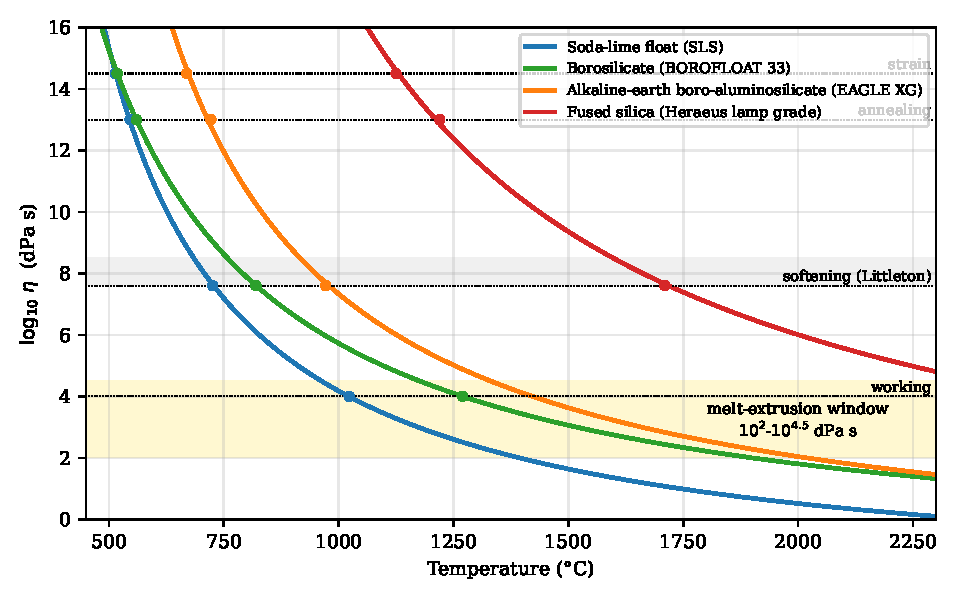
\includegraphics[width=\linewidth]{fig_vft_viscosity.pdf}
  \caption{Vogel--Fulcher--Tammann viscosity curves of the four glass families used in molten glass AM, fitted to published fixed points (markers): soda-lime float \citep{valleydesign_sls}, BOROFLOAT~33 \citep{schott_borofloat}, EAGLE XG \citep{corning_eaglexg} and lamp-grade fused silica \citep{heraeus_quartz}. Horizontal dotted lines mark the strain, annealing, softening and working points. The shaded band \(10^{2}\)--\(10^{4.5}\)\,dPa\,s is the viscosity window within which gravity-fed and cane-fed melt extrusion operates; it is reached at about \SI{1000}{\celsius} for soda-lime, \SI{1250}{\celsius} for borosilicate, \SIrange{1300}{1400}{\celsius} for boro-aluminosilicate and above \SI{2000}{\celsius} for fused silica, which is why the last is accessible only to laser heating. The fused-silica curve above the softening point is an extrapolation of the fixed-point fit and is consistent with the direct measurements compiled by Doremus \citep{doremus2002}.}
  \label{fig:vft}
\end{figure}

\begin{table}[htbp]
  \centering\small
  \caption{VFT constants (\(\eta\) in dPa\,s, \(T\) in K, \(T_0\) quoted in \si{\celsius}) fitted to manufacturer fixed points, and the temperatures at which each glass reaches the melt-extrusion viscosity \(10^{4}\)\,dPa\,s. Fits with \(A\) fixed at \(-1.93\) (universal \(\eta_\infty\) \citep{mauro2009}) are marked \(^{\dagger}\). Generated by \texttt{scripts/make\_figures.py}.}
  \label{tab:vft}
  \begin{tabular}{@{}lS[table-format=-1.2]S[table-format=5.0]S[table-format=-3.0]S[table-format=4.0]l@{}}
    \toprule
    Glass & {\(A\)} & {\(B\) (K)} & {\(T_0\) (\si{\celsius})} & {\(T(10^{4}\,\mathrm{dPa\,s})\) (\si{\celsius})} & Fixed-point source\\
    \midrule
    Soda-lime float & -2.39 & 5210 & 206 & 1023 & \citep{valleydesign_sls,stern2024cgc}\\
    BOROFLOAT~33 (borosilicate) & -1.68 & 6578 & 112 & 1270 & \citep{schott_borofloat}\\
    EAGLE XG (boro-aluminosilicate)\(^{\dagger}\) & -1.93 & 6947 & 250 & {1300--1420 (extrap.)} & \citep{corning_eaglexg}\\
    Fused silica (lamp grade)\(^{\dagger}\) & -1.93 & 13351 & 317 & {\(>\)2000 (extrap.)} & \citep{heraeus_quartz,doremus2002}\\
    \bottomrule
  \end{tabular}
\end{table}

Two practical consequences follow from \cref{fig:vft}. First, the \emph{working range}, defined by Evenline as the interval between working and softening points, is remarkably constant at \SI{295 +- 12}{\celsius} across six soda-lime compositions from studio batch to recycled float \citep{stern2024cgc}. This is why a single crucible-fed machine can be recalibrated for a new soda-lime source by ``viscosity matching'': setting the two VFT expressions equal and solving for the temperature of the new glass that gives the same viscosity as a proven set point,
\begin{equation}
  T_2 = T_{0,2} + \frac{B_2\,(T_1 - T_{0,1})}{B_1 + (T_1 - T_{0,1})(A_1 - A_2)},
  \label{eq:viscmatch}
\end{equation}
which predicted an Optifloat set point of \SI{1037}{\celsius} from a Spruce Pine PWV set point of \SI{1023}{\celsius} and produced a part mass within \SI{3.2}{\percent} of prediction at first attempt \citep{stern2024cgc}. Second, the slope \(\mathrm{d}\log_{10}\eta/\mathrm{d}T\) at the working point is about \SI{-0.012}{\per\kelvin} for soda-lime, so a \SI{10}{\celsius} error in nozzle temperature changes the gravity-fed flow rate by roughly \SI{30}{\percent} through \cref{eq:hp} below. Thermal control to \(\pm\)\SI{3}{\celsius} at the nozzle is therefore a hard requirement, not a refinement.

\subsection{Flow through the nozzle: Hagen--Poiseuille gravity feed}
In crucible-fed machines the melt is driven only by its own head. Klein et al.\ showed that with \(\eta \approx 640\,\)Pa\,s, \(\rho \approx \SI{2400}{\kilogram\per\cubic\metre}\), \(d = \SI{10}{mm}\) and \(v \approx \SI{6}{mm/s}\) the Reynolds number is \(Re = \rho v d/\eta \approx 2\times10^{-4}\), so the flow is creeping (Stokes) flow and the Hagen--Poiseuille law applies segment by segment \citep{klein2015,inamura2018}:
\begin{equation}
  Q = \frac{\Delta P}{R}, \qquad R = \sum_i \frac{8\,\eta\, L_i}{\pi r_i^{4}}, \qquad \Delta P = \rho g H .
  \label{eq:hp}
\end{equation}
Because \(R \propto r^{-4}\), more than half of the total resistance of the G3DP crucible--nozzle assembly resided in the final \SI{10}{mm} bore, and a head of \(H = \SI{80}{mm}\) (\(\Delta P \approx \SI{3.6}{kPa}\)) gave a linear exit velocity of \SI{5.7}{mm/s} \citep{klein2015}. G3DP2 lengthened the nozzle for insulation but widened it to obtain a net \SI{17}{\percent} lower resistance and doubled the head, more than doubling the flow to \SI{5.2}{kg/h} (\SI{570}{mm^3/s}) \citep{inamura2018}. The linear dependence of \(Q\) on \(H\) is also the principal source of drift in gravity-fed printing: as the crucible empties, the bead narrows, which is why G3DP required refilling every few minutes and why G3DP2 raised the reservoir-to-print-volume ratio from \SI{4.6}{\percent} to \SI{29}{\percent} \citep{inamura2018}. Cane-fed and filament-fed machines avoid this problem entirely because the volumetric feed rate is set by the feeder motor, \(Q = \pi r_{\mathrm{cane}}^{2} v_{\mathrm{feed}}\), and the extruded bead cross-section then follows from mass conservation, \(A_{\mathrm{bead}} = Q / v_{\mathrm{travel}}\); over-feeding by \SI{50}{\percent} relative to the geometric requirement was found necessary in laser filament printing to obtain good wetting of the previous layer \citep{kth2022bonding}.

\subsection{Capillary instabilities of the molten cord}
A cylinder of liquid of radius \(a\) and surface tension \(\sigma\) is unstable to axisymmetric perturbations of wavelength \(\lambda > 2\pi a\) (Plateau's criterion). Rayleigh's inviscid analysis \citep{rayleigh1878} gives the growth rate \(\omega\) of a perturbation of wavenumber \(k\) as
\begin{equation}
  \omega^{2} = \frac{\sigma}{\rho a^{3}}\, \frac{x\, I_1(x)}{I_0(x)}\,(1 - x^{2}), \qquad x = ka,
  \label{eq:rayleigh}
\end{equation}
with \(I_n\) the modified Bessel functions. The fastest-growing mode is at \(x \simeq 0.697\), i.e.
\begin{equation}
  \lambda_{\mathrm{opt}} \simeq 9.02\,a \simeq 4.51\, d_{\mathrm{filament}},
  \label{eq:lambdaopt}
\end{equation}
the classical result that a jet breaks into drops spaced by about four and a half diameters \citep{rayleigh1878,tomotika1935,wiki_plateau}. For molten glass, however, the relevant limit is the opposite one. The Ohnesorge number \(Oh = \eta/\sqrt{\rho\sigma a}\) for a \SI{10}{mm} soda-lime cord at \SI{1000}{\celsius} (\(\eta \approx 10^{3}\,\)Pa\,s, \(\sigma \approx \SI{0.32}{\newton\per\metre}\), \(\rho = \SI{2400}{\kilogram\per\cubic\metre}\)) is of order \(10^{3}\), and for a \SI{200}{\micro\metre} fused-silica fibre at \SI{2000}{\celsius} (\(\eta \approx 10^{4.5}\,\)Pa\,s) it is of order \(10^{6}\). Inertia is irrelevant and the Stokes-limit dispersion relation for a viscous thread \citep{tomotika1935} applies,
\begin{equation}
  \omega = \frac{\sigma}{2\eta a}\;\frac{1 - x^{2}}{x^{2}\,[I_0(x)/I_1(x)]^{2} - x^{2} - 1},
  \qquad \omega(x\to 0) \to \frac{\sigma}{6\,\eta\, a},
  \label{eq:tomotika}
\end{equation}
which has no interior maximum: the growth rate increases monotonically toward long wavelengths and its magnitude is set by the visco-capillary time \(\tau_{vc} = \eta a/\sigma\). \Cref{fig:rp} contrasts the two limits. For the G3DP cord \(\tau_{vc} \approx 10^{3}\times 5\times10^{-3}/0.32 \approx \SI{16}{s}\) at the nozzle exit, growing to \(10^{5}\)\,s within a few layers as the glass cools by \SI{350}{\celsius}; capillary break-up therefore never occurs, but the same visco-capillary time governs the \emph{healing} of the layer seam by surface tension. For the laser-heated fibre \(\tau_{vc} \approx 3\times10^{4}\times10^{-4}/0.3 \approx \SI{10}{s}\), and the process must indeed avoid dwell times of this order at full temperature or the free length of fibre between feeder and melt pool necks and separates---the ``premature filament detachment'' failure mode reported for digital glass forming \citep{dgf2026control}.

\begin{figure}[htbp]
  \centering
  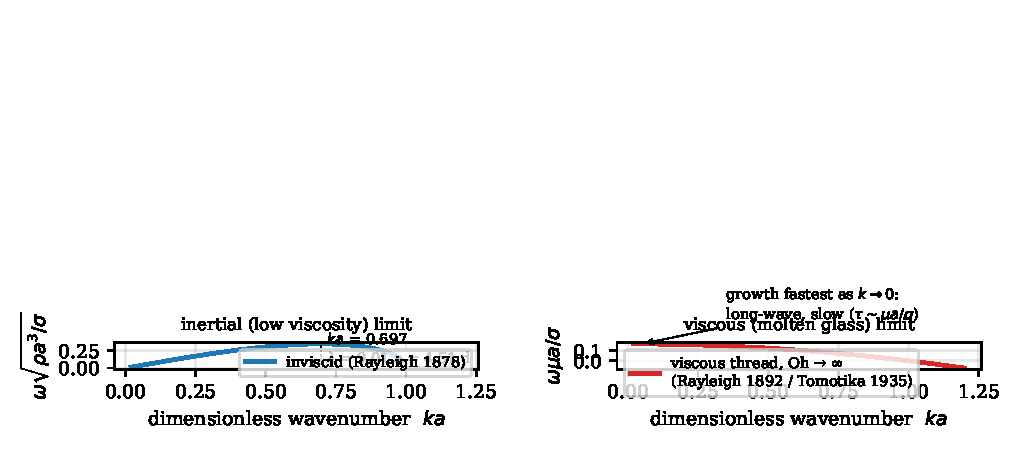
\includegraphics[width=\linewidth]{fig_rayleigh_plateau.pdf}
  \caption{Dispersion relations for the capillary instability of a liquid cylinder. Left: inviscid Rayleigh limit, \cref{eq:rayleigh}, with the most unstable wavelength \(\lambda_{\mathrm{opt}} = 4.51\,d\) marked. Right: Stokes (viscous-thread) limit, \cref{eq:tomotika}, relevant to molten glass cords for which \(Oh \gg 1\): the growth rate scales as \(\sigma/(\eta a)\) and is largest for the longest wavelengths, so break-up is slow and the deposited cord is preserved, but the same time scale controls seam healing. Sources: \citet{rayleigh1878,tomotika1935}.}
  \label{fig:rp}
\end{figure}

\subsection{Gravitational slump and the viscous-thread (coiling) instability}
Slumping of a freshly deposited cord under gravity is a competition between the gravitational stress \(\rho g h\) over a wall of height \(h\) and the viscous resistance; the characteristic sag velocity is \(v_{\mathrm{sag}} \sim \rho g h a^{2}/\eta\). With \(h = \SI{5}{mm}\), \(a = \SI{5}{mm}\) and \(\eta = 10^{3}\,\)Pa\,s this is \SI{3}{mm/s} at the nozzle exit and falls to \SI{3}{\micro\metre/s} once the viscosity has risen five decades: the wall is self-supporting only because the cooling is fast relative to the layer time. This is the origin of the empirical overhang limit of \SIrange{30}{35}{\degree} and the minimum turning radius of \SIrange{6}{15}{mm} of the G3DP machines \citep{klein2015,mit2024masonry}, and of the maximum layer height of \SI{5}{mm} at a \SI{10}{mm/s} feed rate.

When the nozzle is lifted well above the bed, the falling cord buckles and coils, the ``fluid-mechanical sewing machine''. Brun et al.\ rationalised the patterns (meanders, alternating loops, translated coiling) in terms of the dimensionless fall height \(H = H^{*}(g/\nu^{2})^{1/3}\) and belt speed \(V = V^{*}/(g\nu)^{1/3}\), with \(\nu\) the kinematic viscosity, and used a geometrical model to program the coiling of molten soda-lime glass at \SI{1070}{\celsius} into uniformly sized building blocks \citep{brun2017,klein2015}. A G3DP cylinder printed at \(H^{*} = \SI{100}{mm}\) (\(H = 1.02\), \(V = 0.003\)) reproduced translated coiling with loops of consistent radius and pitch, verified by micro-computed tomography \citep{klein2015}. The same instability is now exploited on polymer printers to make graded foams \citep{vti2022}; in glass it offers a route to multiscale lattices whose optical scattering is set by the coil pitch rather than by the layer height.

\subsection{Surface tension, Marangoni flow and wetting}
Surface tension of soda-lime melts is \SIrange{0.31}{0.33}{\newton\per\metre} between \SI{1200}{\celsius} and \SI{1400}{\celsius}, and its temperature coefficient is small and, unusually, positive for many complex silicate liquids \citep{fluegel2007}. In crucible-fed extrusion the temperature gradients across the cord are modest and Marangoni stresses are negligible compared with viscous stresses; the dominant interfacial effect is instead \emph{wetting of the nozzle face}. Molten glass adheres to the alumina nozzle tip, and when the adhering film is asymmetric it exerts an off-axis pull on the just-deposited cord, distorting the wall at convexity changes; G3DP2 reduced this by raising the nozzle tip cone angle from \SIrange{30}{45}{\degree} to reduce the contact area \citep{inamura2018}. In laser melt pools the situation is reversed: intensity gradients of the focused beam produce surface-temperature gradients of \(10^{3}\)--\(10^{4}\)\,K/mm, and Marangoni convection and evaporation recoil determine the melt-pool shape and the surface topography of laser-formed optical glass \citep{machines2026meltpool}. Excess laser power in fibre printing produces visible fumed-silica deposits from vapour condensation, whereas insufficient power leaves ``wiggly'' lines because the fibre does not wet the substrate \citep{kth2022bonding}. Bonding width (the wetted contact width between a \SI{196}{\micro\metre} fibre and a fused-quartz substrate) rises with laser power from \SI{17}{\micro\metre} and saturates near \SI{221}{\micro\metre}, while layer-to-layer bonding widths of \SI{99 +- 12}{\micro\metre} were obtained in 105-layer walls \citep{kth2022bonding}.

\subsection{Transient heat transfer and cooling of the deposited cord}
A deposited cord loses heat by radiation and convection to the chamber and by conduction into the layer below. For a cord of diameter \(d\) whose Biot number is small (\(Bi = h_{\mathrm{eff}} d / 2k \lesssim 0.3\), which holds for \(d \lesssim \SI{15}{mm}\) with \(k \approx \SI{1.4}{\watt\per\metre\per\kelvin}\) and radiative \(h_{\mathrm{eff}} \approx \SIrange{50}{100}{\watt\per\square\metre\per\kelvin}\) at \SI{1000}{\celsius}), a lumped energy balance gives
\begin{equation}
  \rho c_p \frac{d}{4}\,\frac{\mathrm{d}T}{\mathrm{d}t} = -\,h\,(T - T_\infty) - \varepsilon\sigma_{\mathrm{SB}}\,(T^{4} - T_\infty^{4}),
  \label{eq:cooling}
\end{equation}
with emissivity \(\varepsilon \approx 0.9\) for glass in the thermal infrared. \Cref{fig:cooling} integrates \cref{eq:cooling} for soda-lime cords of \SIrange{2}{15}{mm} released at \SI{1050}{\celsius} into a chamber at \SI{520}{\celsius} (crucible-fed architecture) and into ambient air (cane-fed desktop architecture). Two regimes emerge. In the heated chamber a \SI{10}{mm} cord falls below the softening point in about \SI{25}{s} and then asymptotes to the chamber temperature, never entering the stress-generating region below the annealing point until the programmed anneal; this reproduces the measured \SI{350}{\celsius} drop across five layers at a \SI{4.5}{mm}, \SI{6}{mm/s} layer schedule (about \SI{50}{s} per layer for a \SI{300}{mm} perimeter) \citep{klein2015}. In open air a \SI{2}{mm} cane-fed filament crosses the softening point in \SI{2}{s} and the annealing point in \SI{4}{s}; the part is therefore built as an already rigid, stressed body, which is why cane-fed desktop machines rely on rapid solidification for overhangs and bridges \citep{maple_ammedia} but must anneal afterwards, and why their wall thicknesses are limited to a few millimetres. For 1-D conduction into a semi-infinite substrate the interface temperature after contact is the contact temperature \(T_c = (T_1 e_1 + T_2 e_2)/(e_1 + e_2)\) with effusivities \(e = \sqrt{k\rho c_p}\); for glass on glass this is simply the mean of cord and previous-layer temperatures, so a \SI{990}{\celsius} cord landing on a \SI{700}{\celsius} layer produces an \SI{845}{\celsius} interface (\(\eta \approx 10^{5}\)\,dPa\,s)---fluid enough to fuse, which is consistent with the SEM observation of a blunt, featureless interlayer interface in annealed G3DP samples \citep{klein2015}.

\begin{figure}[htbp]
  \centering
  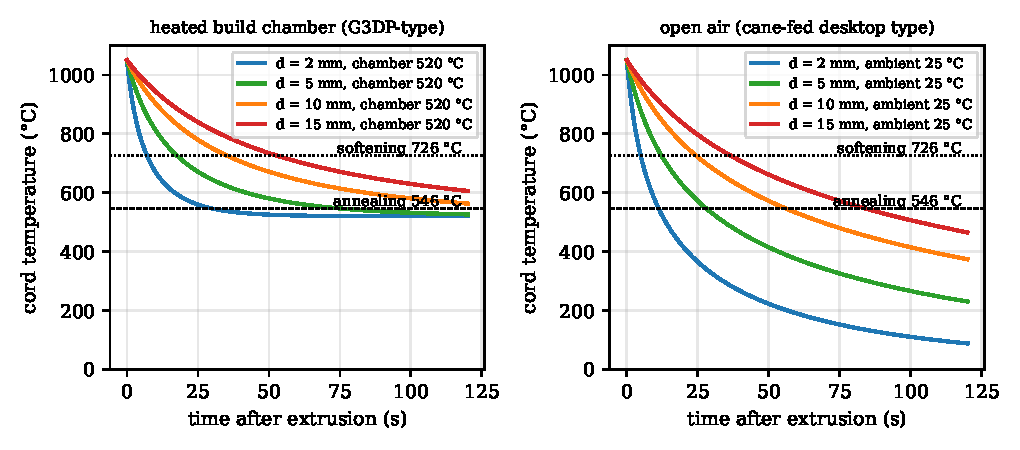
\includegraphics[width=\linewidth]{fig_cord_cooling.pdf}
  \caption{Lumped radiative--convective cooling, \cref{eq:cooling}, of soda-lime cords of \SI{2}{}--\SI{15}{mm} diameter released at \SI{1050}{\celsius} (\(\rho=\SI{2500}{\kilogram\per\cubic\metre}\), \(c_p=\SI{1200}{\joule\per\kilogram\per\kelvin}\), \(\varepsilon=0.9\), \(h=\SI{15}{\watt\per\square\metre\per\kelvin}\)). Left: into a build chamber at \SI{520}{\celsius}, as in the G3DP family; the cord stays above the annealing point. Right: into ambient air, as in cane-fed desktop printers; thin filaments pass through the transformation range within seconds and accumulate residual stress that must be removed by a post-anneal. The softening (\SI{726}{\celsius}) and annealing (\SI{546}{\celsius}) points of float glass are marked.}
  \label{fig:cooling}
\end{figure}

In laser filament processes the energy balance is local. Luo et al.\ estimated melt-pool temperature from a low-order balance between absorbed laser power, radiative loss and conduction along the filament and into the substrate, validated against incandescence spectra; the model predicts the onset of ``reboil'' (bubble nucleation from dissolved gases and sulfate decomposition) above a threshold temperature and the incomplete fusion (index inhomogeneity) below it \citep{luo2017heat,luo2017sodalime}. For fused silica the window is bounded below by roughly \SI{1900}{\celsius} for wetting and above by evaporation, which becomes measurable near \SI{2200}{\celsius} \citep{witzendorff2018,kth2022bonding}. Because the thermal conductivity of glass is low, heat delivered to the top of a thick filament diffuses slowly to the interface; injecting the laser from the side so that it heats the filament--substrate junction directly was shown to raise the achievable deposition rate \citep{capps2021interface}.

\subsection{Thermal stress and the annealing requirement}
When a glass wall cools through the transformation range with a through-thickness temperature difference \(\Delta T\), the frozen-in stress is of order
\begin{equation}
  \sigma_{\mathrm{res}} \approx \frac{E\,\alpha\,\Delta T}{2(1-\nu_{\mathrm{P}})},
  \label{eq:stress}
\end{equation}
which for soda-lime (\(E = \SI{70}{GPa}\), \(\alpha = \SI{9e-6}{\per\kelvin}\), \(\nu_{\mathrm{P}} = 0.22\)) is \SI{40}{MPa} per \SI{100}{\celsius}---comparable to the practical tensile strength of glass (\SIrange{40}{80}{MPa}) \citep{inamura2018}. This is why samples printed at room temperature in the first G3DP experiments showed radial residual stress under the polariscope and a flexural strength one fifth of that of samples printed into the heated chamber \citep{klein2015}, and why fused silica, with \(\alpha = \SI{0.5e-6}{\per\kelvin}\), tolerates the extreme gradients of laser deposition that would shatter soda-lime or borosilicate \citep{luo2018quartz,lgd2021coaxial}. The annealing schedule is set by the relaxation time \(\tau = \eta/G\) (\(G \approx \SI{30}{GPa}\)): \SI{15}{min} at the annealing point, hours at the strain point, and a cooling rate below it that keeps \(\Delta T\) small; Evenline's masonry units of \SI{13}{mm} wall thickness were annealed with schedules of several hours, and the fully printed variants with thicker bases required longer cycles \citep{mit2024masonry}.
